\chapter{A multitude of tests}

\epigraph{Science is what we understand well enough to explain to a computer. Art is everything else we do.}{Donald E. Knuth}

\blindtext

\begin{figure}
    \small
    \centering
    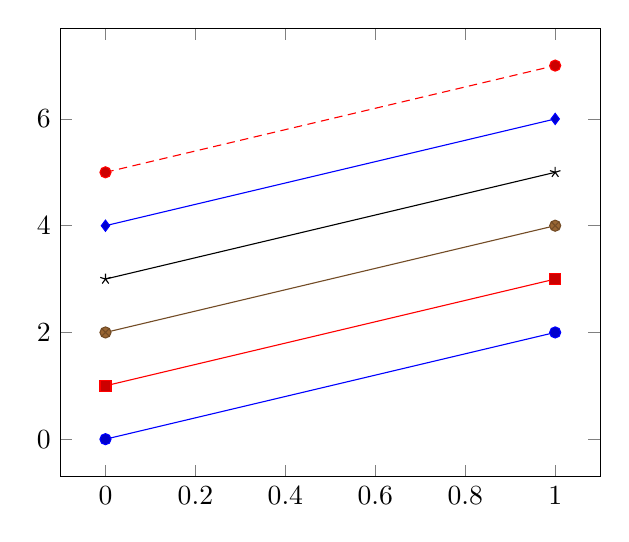
\begin{tikzpicture}
       \begin{axis}
          \addplot coordinates{(0,0) (1,2)};
          \addplot coordinates{(0,1) (1,3)};
          \addplot coordinates{(0,2) (1,4)};
          \addplot coordinates{(0,3) (1,5)};
          \addplot coordinates{(0,4) (1,6)};
          \addplot coordinates{(0,5) (1,7)};
       \end{axis}
    \end{tikzpicture}
    \caption{Just a fancy test for auto-coloring of graphs}
\end{figure}

\section{Some math}

\marginnote{This formula is also known as \emph{Pythagorean Theorem}, albeit it is usually written with the variables $a$, $b$, and $c$.}
Here follows some tests for typesetting math. Note how we use the \texttt{\\marginnote} command to add some pretty notes which appear in the margin. This is quite nice, as it allows a more narrow width of the text body without the page looking too sparse\footnote{This is a footnote}. Here comes our first equation
\begin{align}
  z^2 &= x^2 + y^2 \\
  z &= \sqrt{x^2 + y^2} \,.
\end{align}

\pagebreak
\marginnote{Did you know? The discrete fourier transformation shown in equation \cref{eqn:dft} is the backbone of the modern information-society.}
And here comes some more math, this time a discrete Fourier transformation (DFT)  which is a little bit more sophisticated than the last example\footnote{More is always better!}:
\begin{align}
	f_m =  \sum_{k=0}^{2n-1} x_k \, e^{-\frac{2\pi i}{2n} mk } \label{eqn:dft}
\qquad
m = 0,\dotsc,2n-1 \,.
\end{align}
For words of science, see~\cite{botsch2010polygon}. Unfortunately, that book has nothing about wolves.

\begin{figure}
	\small
	\centering
	\begin{tikzpicture}
		\begin{axis}[
			axis lines=left,
			scaled ticks=false,
			xticklabel style={
				rotate=90,
				anchor=east,
				/pgf/number format/precision=3,
				/pgf/number format/fixed,
				/pgf/number format/fixed zerofill,
			},
		]
		% density of Normal distribution:
		\newcommand\MU{0}
		\newcommand\SIGMA{0.1}
		\addplot+[mark=none,domain=-3*\SIGMA:3*\SIGMA,samples=201]
		{exp(-(x-\MU)^2 / 2 / \SIGMA^2)
			/ (\SIGMA * sqrt(2*pi))};
		\end{axis}
	\end{tikzpicture}
	\caption{Gaussian distribution. This plot shows a guassian distribution with mean $\mu = 0$ and standard deviation $\sigma = 0.1$. As clearly visible, the value of the distribution never reaches zero.}
	\label{fig:gaussian_distr}
\end{figure}

\section{Even more tests}
\marginnote{Blood-red were his spurs i' the golden noon; wine-red was his velvet coat, when they shot him down on the highway, down like a dog on the highway, and he lay in his blood on the highway, with the bunch of lace at his throat.}
\blindtext
\todo{write thesis}

\subsection{A test of three parts}
\blindtext

\subsection{And a second subsection}
\Blindtext
